\section{Lineaire regressie met meerdere variabelen}

\subsection{Lineair model met meerdere variabelen}
We kunnen de lineaire regressie die we tot nu toe behandeld hebben uitbreiden om meerdere \textit{features} te betrekken in ons model. We gebruiken in dit geval $x^{(i)}$ om de \textit{features} van het $i^{de}$ trainingsvoorbeeld voor te stellen en $x^{(i)}_{j}$ om de waarde van \textit{feature} $j$ in het $i^{de}$ trainingsvoorbeeld voor te stellen. Formule \ref{eq:f-wb} wordt dan uitgebreid tot:
\begin{equation}
	f_{\vec{w},b}(\vec{x}^{(i)}) = \vec{w} \cdot \vec{x} + b = \vec{w}^{T} \vec{x} + b = w_{1}x_{1} + w_{2}x_{2} + \ldots + w_{n}x_{n} + b
	\label{eq:f-wb-multi}
\end{equation}
\noindent
Hierbij bevat de vector $\vec{x}$ de \textit{features} en vector $\vec{w}$ de gewichten. Beide vectoren zijn kolomvectoren. 

\subsection{Vectorisatie in Python}

We kunnen deze formule gemakkelijk uitrekenen met behulp van NumPy in Python. We moeten wel rekening houden met het feit dat de indexatie dan begint vanaf index 0 en niet vanaf index 1 zoals dit in de lineaire algebra is. Dit kunnen we, want we zijn niet achterlijk. Aangezien onze vectoren groot kunnen worden, werken we best met vectorisatie om zo efficiënt mogelijk te werken. In Python kunnen we gebruik maken van `\textit{numpy.dot}' om het scalair of dot product uit te werken. \\

\begin{lstlisting}
	# Declaratie van parameters en features
	w = np.array([1.0, 2.5, -3.3])
	b = 4
	x = np.array([10, 20, 30])
	
	# Zonder vectorisatie
	f = w[0] * x[0] + 
	    w[1] * x[1] + 
	    w[2] * x[2] + b
	
	# Zonder vectorisatie
	f = 0
	for j in range(0,n) : 
	    f = f + w[j] * x[j]
	f = f + b
	
	# Met vectorisatie
	f = np.dot(w,x) + b
\end{lstlisting}

\subsection{Kostfunctie met meerdere variabelen}

De formule voor de kostfunctie (formule \ref{eq:cost-function}) kunnen we ook uitbreiden om met meerdere \textit{features} om te gaan. We bekomen dan:
\begin{equation}
	J(\vec{w}, b) = \frac{1}{2m}\sum_{i=1}^{m}(f_{\vec{w},b}(\vec{x}^{(i)}) - y^{(i)})^{2}
	\label{eq:cost-function-multi}
\end{equation}
\noindent
Dit is in principe dezelfde formule als voordien, alleen hebben we nu $n+1$ parameters in plaats van 2, waarbij $n$ het aantal \textit{features} is.

\subsection{\textit{Gradient descent} met meerdere variabelen}

\subsubsection{\textit{Gradient descent}}

Vervolgens kunnen ook de formules voor \textit{gradient descent} aangepast worden. Dit leidt tot volgende formules:

\begin{equation}
	w_{j} = w_{j} - \alpha \frac{\partial}{\partial w_{j}} J(\vec{w}, b) = w_{j} - \alpha \frac{1}{m}\sum_{i=1}^{m}[(f_{\vec{w},b}(\vec{x}^{(i)}) - y^{(i)})x^{(i)}_{j}]
	\label{eq:gradient-descent-lin-reg-multi-w}
\end{equation}
\begin{equation}
	b = b - \alpha \frac{\partial}{\partial b} J(\vec{w}, b) = b - \alpha \frac{1}{m}\sum_{i=1}^{m}[(f_{\vec{w},b}(\vec{x}^{(i)}) - y^{(i)})]
	\label{eq:gradient-descent-lin-reg-multi-b}
\end{equation}
\noindent
We zullen $b$ en $w_{j}$ nog steeds simultaan updaten voor $j = 1...n$, maar dit is ter vereenvoudiging weggelaten hier.

\subsubsection{Feature scaling}

Wanneer onze features een verschillende range hebben, kan dit leiden tot trage convergentie. We kunnen dit versnellen door \textit{feature scaling} toe te passen zodat alle features dezelfde range krijgen. Figuur \ref{fig:feature-scaling} toont het resultaat hiervan.

\begin{figure}[h]
	\centering
	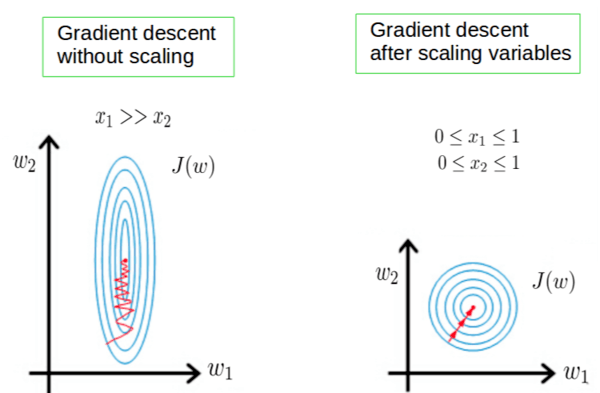
\includegraphics[width=0.75\textwidth]{images/8-feature-scaling.png}
	\caption{Effect van feature scaling}
	\label{fig:feature-scaling}
\end{figure}
\noindent
Er kan op meerdere manieren genormaliseerd worden. Een eerste optie is om de \textit{features} simpelweg te delen door hun maximumwaarde. Dit levert een range tussen 0 en 1 op. Een andere manier is Z-score normalisatie. Hierbij vervangen we $x_{i}$ door $\frac{x_{i} - \mu_{i}}{\sigma_{i}}$. Dit levert een range tussen -3 en 3 op. 

\subsubsection{Learning rate}

We willen natuurlijk ook een manier hebben om te bepalen of onze \textit{learning rate} $\alpha$ correct ingesteld is. Dit kan bijvoorbeeld met een automatische convergentie test waarbij we kijken of de kostfunctie monotoon daalt als we blijven itereren. We kunnen spreken van convergentie als $J(\vec{w},b)$ met minder dan $10^{-3}$ daalt in één iteratie. Wanneer $J(\vec{w},b)$ stijgt in plaats van daalt (divergeert) of afwisselend daalt en stijgt, is onze waarde voor $\alpha$ te groot. Wanneer $\alpha$ te klein is zullen we trage convergentie hebben. In dit geval kan het interessanter zijn om de hyperparameter iets groter te maken. 

\subsection{Feature Engineering}

\subsubsection{Feature Engineering}

Bij \textit{feature engineering} gaan we nieuwe \textit{features} maken op basis van domeinkennis en intuïtie door bestaande \textit{features} te transformeren en combineren. Dit wordt vooral toegepast bij kleine datasets.

\subsubsection{Polynomiale regressie}

Bij polynomiale regressie zullen we van ons eerstegraads model overschakelen naar een meergraads model dat beter aansluit door onze oorspronkelijke \textit{feature} tot een macht te verheffen en deze als extra feature te gebruiken. Hier is het wel belangrijk om aan \textit{feature scaling} te doen zodat onze convergentie niet te traag gaat bij \textit{gradient descent}.
